% Обзор отраслевого отчета "Топ-40 стран-импортеров меда (ТН ВЭД 040900), объем в тоннах"
% Нативный LaTeX Beamer, стиль повторяет эталонный шаблон: синий #3333B2,
% плашка frametitle во всю ширину, скругленный баннер с тенью, круглые буллеты,
% booktabs-таблицы, номер страницы N / M. Компилировать XeLaTeX (2 прохода).
\documentclass{beamer}

\usepackage{fontspec}
\setsansfont{CMU Sans Serif}

\usepackage{booktabs}
\usepackage{array}
\usepackage{pgfplots}
\pgfplotsset{compat=newest}

\emergencystretch=2.5em

\definecolor{accblue}{RGB}{51,50,178}
\definecolor{srcgray}{RGB}{102,102,102}

\setbeamercolor{structure}{fg=accblue}
\setbeamercolor{normal text}{fg=black, bg=white}
\setbeamercolor{frametitle}{bg=accblue, fg=white}
\setbeamercolor{banner}{bg=accblue, fg=white}
\setbeamercolor{pageno}{fg=black!60}

\setbeamertemplate{navigation symbols}{}
\setbeamertemplate{itemize items}[circle]

% плашка заголовка во всю ширину слайда
\setbeamertemplate{frametitle}{%
  \nointerlineskip
  \begin{beamercolorbox}[wd=\paperwidth,sep=0.55em]{frametitle}%
    \hspace*{0.42cm}{\bfseries\fontsize{16}{20}\selectfont\insertframetitle}%
  \end{beamercolorbox}%
}

% номер страницы N / M
\setbeamertemplate{footline}{%
  \begin{beamercolorbox}[wd=\paperwidth,ht=2.2ex,dp=1.1ex,rightskip=3mm]{pageno}%
    \hfill{\scriptsize\insertframenumber\,/\,\inserttotalframenumber}%
  \end{beamercolorbox}%
}

\title{Обзор отраслевого отчета "Топ-40 стран-импортеров меда (ТН ВЭД 040900), объем в тоннах"}
\author{Команда 10130}
\date{25 ноября 2026 г.}

\begin{document}

% ── 1. Титульный ─────────────────────────────────────────────────────────────
\begin{frame}[plain]
  \centering
  \vspace{2mm}
  {\small Курс "Поиск экспортных рынков"~ · ~Команда 10130\par}
  \vfill
  \makebox[\textwidth][c]{%
    \begin{beamercolorbox}[wd=0.95\paperwidth,center,rounded=true,shadow=true,sep=10pt]{banner}
      {\bfseries\fontsize{16}{21}\selectfont
       Обзор отраслевого отчета\\
       "Топ-40 стран-импортеров меда\\
       (ТН ВЭД 040900), объем в тоннах"\par}
    \end{beamercolorbox}%
  }\par
  \vfill
  {\small Платформа GTAIC (издатель EXPORT HUNTER, UAB, Вильнюс), 217 страниц, сгенерирован 24.11.2026\par}
  \vfill
  {\small 25 ноября 2026 г.\par}
  \vspace{2mm}
  \note{Здравствуйте. Мы, команда 10130, курса "Поиск экспортных рынков", представляем обзор отраслевого отчета платформы GTAIC о сорока крупнейших импортерах натурального меда. За пять минут покажем: что это за отчет и на каких данных он построен, что происходит с мировым рынком, кто главные покупатели и поставщики, как отчет соотносится с нашими расчетами и что мы из него возьмем для исследования экспорта в США, Японию и Южную Корею.}
\end{frame}

% ── 2. Паспорт и методология ─────────────────────────────────────────────────
\begin{frame}[t]
  \frametitle{Паспорт и методология отчета}
  {\footnotesize
  \begin{columns}[t]
    \begin{column}{0.47\textwidth}
      \textbf{Данные и охват}
      \begin{itemize}
        \item Базы: UN Comtrade (свыше 200 стран), Eurostat Comext, таможня Китая GACC
        \item Топ-40 импортеров - 96,07~\% мирового импорта в тоннах
        \item Измерители: стоимость (млн долл.), тоннаж (тыс. т), цена-прокси CIF (долл./т)
        \item Периоды: календарные 2020-2025, частичный 2026*, LTM-окна по странам
      \end{itemize}
    \end{column}
    \begin{column}{0.47\textwidth}
      \textbf{Пометки достоверности}
      \begin{itemize}
        \item У 5 стран тоннаж - зеркальная реконструкция по партнерам
        \item Китай, Республика Корея*, ЮАР - официальный флаг недостоверности тоннажа (аномалии цен CIF)
        \item LTM-окна стран не синхронизированы: разброс до 5 месяцев
        \item Цена-прокси отражает и сортовую структуру поставок
      \end{itemize}
    \end{column}
  \end{columns}}
  \vfill
  {\scriptsize\color{srcgray} Источник: GTAIC (2026), стр. 1-13. LTM (last twelve months) - 12 месяцев, предшествующих дате генерации. Единицы: млн долл., тыс. т, долл./т.\par}
  \note{Отчет сгенерирован 24 ноября 2026 года на данных ООН, Евростата и китайской таможни, объем - 217 страниц. Покрывает сорок стран, на которые приходится 96 процентов мирового импорта в тоннах. Два измерителя: деньги и тонны, плюс цена-прокси. Три методологические оговорки: окна стран не синхронизированы, у пяти стран тоннаж реконструируется зеркально, а Китай, Корея и ЮАР помечены официальными флагами недостоверности.}
\end{frame}

% ── 3. Динамика рынка ────────────────────────────────────────────────────────
\begin{frame}[t]
  \frametitle{2025 год: рекорд по тоннажу, в деньгах ниже пика 2022 года}
  {{\color{accblue}\bfseries 776,05~тыс.~т} (+2,1~\%) при {\color{accblue}\bfseries 2,32~млрд~долл.} (+8,0~\%); средняя цена-прокси 2\,983~долл./т - на 11~\% ниже денежного пика 2022 года\par}
  \smallskip
  \begin{columns}[t]
    \begin{column}{0.48\textwidth}
      {\small\bfseries Импорт, млрд долл.}\par\smallskip
      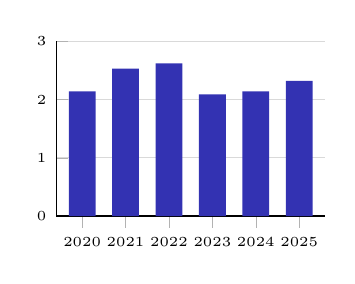
\begin{tikzpicture}
        \begin{axis}[width=50mm, height=38mm, ybar, bar width=3.4mm,
            ymin=0, ymax=3, ytick={0,1,2,3},
            symbolic x coords={2020,2021,2022,2023,2024,2025}, xtick=data,
            enlarge x limits=0.12,
            ymajorgrids, grid style={gray!30},
            axis lines*=left, tick label style={font=\tiny},
            tick style={gray!60}]
          \addplot[draw=none, fill=accblue] coordinates
            {(2020,2.14) (2021,2.53) (2022,2.62) (2023,2.09) (2024,2.14) (2025,2.32)};
        \end{axis}
      \end{tikzpicture}
    \end{column}
    \begin{column}{0.48\textwidth}
      {\small\bfseries Тоннаж, тыс. т}\par\smallskip
      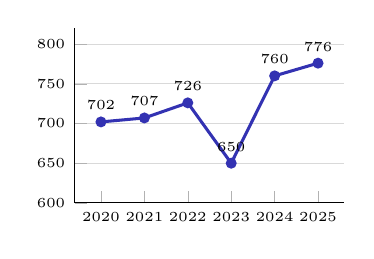
\begin{tikzpicture}
        \begin{axis}[width=50mm, height=38mm,
            ymin=600, ymax=820, ytick={600,650,700,750,800},
            symbolic x coords={2020,2021,2022,2023,2024,2025}, xtick=data,
            enlarge x limits=0.12,
            ymajorgrids, grid style={gray!30},
            axis lines*=left, tick label style={font=\tiny},
            tick style={gray!60},
            nodes near coords, every node near coord/.append style=
              {font=\tiny, color=black, anchor=south, yshift=0.5pt}]
          \addplot[accblue, line width=1.1pt, mark=*, mark size=1.4pt] coordinates
            {(2020,702) (2021,707) (2022,726) (2023,650) (2024,760) (2025,776)};
        \end{axis}
      \end{tikzpicture}
    \end{column}
  \end{columns}
  \vfill
  {\scriptsize\color{srcgray} Рис.~1-2. Источник: GTAIC (2026), табл.~2, рис.~14-16. Период: календарные 2020-2025~гг. Единицы: млрд долл., тыс. т.\par}
  \note{Главное событие 2025 года - исторический максимум физического импорта: 776 тысяч тонн, плюс два процента к 2024 году. В деньгах рынок вырос до 2,32 миллиарда долларов, но это все еще на 11 процентов ниже пика 2022 года. Вывод: рынок восстанавливается объемами, в основном в массовых ценовых сегментах - средняя цена снизилась примерно до 2 983 долларов за тонну.}
\end{frame}

% ── 4. Крупнейшие импортеры ──────────────────────────────────────────────────
\begin{frame}[t]
  \frametitle{Крупнейшие импортеры: США - треть мирового рынка}
  {На пятерку лидеров приходится 58,0~\% стоимости 2025 года; 27 из 40 рынков отчета - европейские\par}
  \smallskip
  \begin{columns}[t]
    \begin{column}{0.38\textwidth}
      \begin{tikzpicture}
        \begin{axis}[width=38mm, height=44mm, xbar, bar width=3.4mm,
            xmin=0, xmax=800, xtick={0,200,400,600,800},
            symbolic y coords={Франция,Великобритания,Япония,Германия,США}, ytick=data,
            enlarge y limits=0.12,
            xmajorgrids, grid style={gray!30},
            axis lines*=left, tick label style={font=\tiny},
            tick style={gray!60}]
          \addplot[draw=none, fill=accblue] coordinates
            {(736.33,США) (263.78,Германия) (142.32,Япония) (141.64,Великобритания) (127.05,Франция)};
        \end{axis}
      \end{tikzpicture}
    \end{column}
    \begin{column}{0.58\textwidth}
      {\footnotesize\setlength{\tabcolsep}{3pt}
      \begin{tabular}{@{}l r@{}}
        \toprule
        Страна & LTM, млн долл. \\
        \midrule
        США & 736,33 \\
        Германия & 263,78 \\
        Япония & 142,32 \\
        Великобритания & 141,64 \\
        Франция & 127,05 \\
        Респ. Корея* (24-е место) & 19,44 \\
        \bottomrule
      \end{tabular}\par}
    \end{column}
  \end{columns}
  \vfill
  {\scriptsize\color{srcgray} Источник: GTAIC (2026), табл. 51-52 (стр. 64-99). Период: LTM-окна. Единицы: млн долл. США. Звездочка - официальное предупреждение отчета о вероятной недостоверности тоннажа.\par}
  \note{Пятерка крупнейших импортеров: США, Германия, Япония, Великобритания и Франция - вместе 58 процентов мировой стоимости. США - третий мирового рынка: 736 миллионов долларов и около трети мирового тоннажа, и единственный из большой пятерки с устойчивым пятилетним ростом. Обратите внимание: география отчета европоцентрична, 27 из 40 рынков - европейские. Южная Корея, наш целевой рынок, стоит на 24-м месте со звездочкой - к ней вернемся через слайд.}
\end{frame}

% ── 5. США ───────────────────────────────────────────────────────────────────
\begin{frame}[t]
  \frametitle{США: треть мирового рынка и главный драйвер роста}
  \begin{columns}[t]
    \begin{column}{0.30\textwidth}
      {\color{accblue}\bfseries\fontsize{20}{24}\selectfont 736,33\par}
      {\scriptsize\color{black!60} млн долл. LTM (+4,1~\%)\par}
    \end{column}
    \begin{column}{0.30\textwidth}
      {\color{accblue}\bfseries\fontsize{20}{24}\selectfont 29,83~\%\par}
      {\scriptsize\color{black!60} стоимости 2025 года\par}
    \end{column}
    \begin{column}{0.30\textwidth}
      {\color{accblue}\bfseries\fontsize{20}{24}\selectfont +9,36~\%\par}
      {\scriptsize\color{black!60} CAGR импорта, 5 лет\par}
    \end{column}
  \end{columns}
  \medskip
  \begin{itemize}
    \item Тоннаж 264,11~тыс.~т (+1,3~\%) - около трети мирового импорта в тоннах
    \item Поставщики: Аргентина нарастила долю до 25,4~\% (годом ранее 20,0~\%); Индия сократила поставки на 27,4~\% (доля 19,0~\% против 27,2~\%)
    \item Отчет связывает сдвиг поставщиков с антидемпинговыми пошлинами США с июня 2022 г. - цитируем как контекст отчета, а не как проверенную причину
  \end{itemize}
  \vfill
  {\scriptsize\color{srcgray} Источник: GTAIC (2026), табл. 51-52 (стр. 64-99), стр. 213 (торговые меры). Период: LTM; CAGR - 2020-2025 гг. Единицы: млн долл., тыс. т.\par}
  \note{Наш первый целевой рынок - США. Импорт растет и в деньгах, и в тоннах: плюс 4 и плюс 1 процент, а пятилетний рост - 9,4 процента в год, единственный устойчивый среди большой пятерки. Состав поставщиков меняется: Аргентина подняла долю до четверти рынка, Индия потеряла 27 процентов поставок. Отчет связывает это с антидемпинговыми пошлинами 2022 года; мы цитируем это как контекст отчета, а не как проверенную причину.}
\end{frame}

% ── 6. Целевые рынки ─────────────────────────────────────────────────────────
\begin{frame}[t]
  \frametitle{Целевые рынки: Япония и Республика Корея*}
  {\footnotesize
  \begin{columns}[t]
    \begin{column}{0.47\textwidth}
      \textbf{Япония - рисковый рынок}
      \begin{itemize}
        \item 142,32~млн~долл. (-3,4~\%) и 48,32~тыс.~т (-5,7~\%)
        \item Пятилетний CAGR -2,84~\%, самый низкий прогнозный рост среди 40 стран
        \item Иена ослабла со 140,5 до 151,5 иен за доллар
        \item Поставщики: Китай 42,5~\% рынка, Новая Зеландия 18,5~\%
      \end{itemize}
    \end{column}
    \begin{column}{0.47\textwidth}
      \textbf{Республика Корея* - быстрый, но ненадежный}
      \begin{itemize}
        \item 19,44~млн~долл. (+45,6~\%) при тоннаже всего 2,23~тыс.~т
        \item Цена-прокси 8\,704~долл./т - втрое выше средней по рынку (2\,983~долл./т)
        \item Официальный флаг недостоверности тоннажа (аномалия CIF)
        \item Вывод: рост в долларах подтвержден, "взрывной" рост в тоннах - нет
      \end{itemize}
    \end{column}
  \end{columns}}
  \vfill
  {\scriptsize\color{srcgray} Источник: GTAIC (2026), стр. 195 (Япония), стр. 204 (Корея), стр. 12 (LTM-окна). Единицы: млн долл., тыс. т, долл./т.\par}
  \note{Япония - рисковый рынок: единственный крупный рынок с падением сразу по обоим измерителям, минус 3,4 процента в деньгах и минус 5,7 в тоннах. Отчет объясняет это ослаблением иены. Корея - обратный случай: плюс 45,6 процента в долларах, но при тоннаже в 2,2 тысячи тонн расчетная цена выходит втрое выше средней по рынку. Отчет сам помечает корейский тоннаж флагом недостоверности, поэтому рост в долларах подтверждаем, а "взрывной" рост в тоннах - нет.}
\end{frame}

% ── 7. Поставщики ────────────────────────────────────────────────────────────
\begin{frame}[t]
  \frametitle{Поставщики: концентрация тоннажа и большой ценовой разрыв}
  {\small
  \begin{tabular}{@{}l r r r@{}}
    \toprule
    Поставщик & млн долл. & Доля, \% & Цена, долл./т \\
    \midrule
    Аргентина & 293,76 & 12,02 & 2\,578 \\
    Новая Зеландия & 288,30 & 11,79 & 20\,810 \\
    Китай & 231,05 & 9,45 & 1\,438 \\
    Индия & 184,61 & 7,55 & 1\,783 \\
    Украина & 143,85 & 5,88 & 3\,088 \\
    \bottomrule
  \end{tabular}\par}
  \medskip
  \begin{itemize}
    \item Тройка "Китай - Аргентина - Индия" дает 47,0~\% тоннажа, но лишь около 29~\% стоимости
    \item Премия мануки: 18,7~тыс.~долл./т в США (в 6,7 раза выше средней), 45,8~тыс.~долл./т во Франции (в 12 раз)
  \end{itemize}
  \vfill
  {\scriptsize\color{srcgray} Источник: GTAIC (2026), табл. 54, 59, 64 (стр. 110-141). Период: LTM. Единицы: млн долл., \%, долл./т.\par}
  \note{Поставщики: Аргентина первая по стоимости, Новая Зеландия почти догоняет ее за счет дорогой мануки. Рынок высоко концентрирован в физическом измерении: тройка Китай - Аргентина - Индия дает 47 процентов тоннажа, но только около 29 процентов стоимости. Ценовой разрыв огромный: от 1 438 долларов за тонну у Китая до почти 21 тысячи у Новой Зеландии.}
\end{frame}

% ── 8. Сопоставление с BACI ──────────────────────────────────────────────────
\begin{frame}[t]
  \frametitle{Сопоставление с расчетами команды (BACI, 2024)}
  {\small
  \begin{tabular}{@{}l >{\raggedleft\arraybackslash}p{25mm} >{\raggedleft\arraybackslash}p{25mm} >{\raggedleft\arraybackslash}p{23mm}@{}}
    \toprule
    Рынок & BACI 2024, млн долл. & GTAIC LTM, млн долл. & GTAIC тоннаж, тыс. т \\
    \midrule
    США & 621,2 & 736,33 & 264,11 \\
    Япония & 132,2 & 142,32 & 48,32 \\
    Респ. Корея* & 16,5 & 19,44 & 2,23 \\
    \bottomrule
  \end{tabular}\par}
  \medskip
  \begin{itemize}
    \item Направления совпадают по всем трем рынкам: США растут, Япония сокращается, Корея растет
    \item Точные уровни несопоставимы: календарный 2024 г. против несинхронных LTM-окон; доллары против тонн
    \item Ценность отчета для панели - физические объемы и цены, которых нет в долларовой базе BACI
  \end{itemize}
  \vfill
  {\scriptsize\color{srcgray} Источники: расчеты команды по OEC/CEPII BACI, куб trade\_i\_baci\_a\_17, HS6 040900 (ДЗ-5); GTAIC (2026), табл. 51-53. Периоды: календарный 2024 г. и LTM. Единицы: млн долл., тыс. т.\par}
  \note{Мы сверили отчет с собственной панелью BACI за 2024 год. Направления совпадают по всем трем целевым рынкам: США растут, Япония падает, Корея растет. Точные уровни сопоставлять нельзя: у нас календарный год в долларах, у отчета несинхронные двенадцатимесячные окна. Главное - отчет добавляет физические объемы и цены, которых в нашей долларовой панели нет.}
\end{frame}

% ── 9. Оценка отчета ─────────────────────────────────────────────────────────
\begin{frame}[t]
  \frametitle{Оценка отчета: сильные стороны и ограничения}
  {\footnotesize
  \begin{columns}[t]
    \begin{column}{0.47\textwidth}
      \textbf{Сильные стороны}
      \begin{itemize}
        \item Охват 40 рынков - 96,07~\% мирового импорта в тоннах
        \item Тонны и цены-прокси, которых нет в долларовых базах
        \item Официальные флаги недостоверных данных
        \item Единая товарная детализация по поставщикам
      \end{itemize}
    \end{column}
    \begin{column}{0.47\textwidth}
      \textbf{Ограничения}
      \begin{itemize}
        \item LTM-окна не синхронизированы, межстрановые сравнения формально некорректны
        \item "Прогноз" - линейная экстраполяция (Литва +150~\% - эффект малой базы)
        \item Рейтинг: равные веса без нормировки на размер рынка (Франция первая при 4,8~\% рынка)
        \item Пошлины и режимы доступа не учитываются
      \end{itemize}
    \end{column}
  \end{columns}}
  \vfill
  {\scriptsize\color{srcgray} Источник: критическая оценка команды по материалам GTAIC (2026); подробный разбор - в обзоре команды, разд. 6.\par}
  \note{Что отчет дает: полный охват, физические объемы и честные пометки о качестве данных. Чего не дает: окна не синхронизированы, прогноз - это линейная экстраполяция, рейтинг уравнивает страны разного размера и полностью игнорирует пошлины. Поэтому используем отчет как источник фактуры и гипотез, а не как готовые выводы.}
\end{frame}

% ── 10. Выводы ───────────────────────────────────────────────────────────────
\begin{frame}[t]
  \frametitle{Выводы и следующий шаг}
  \begin{itemize}
    \item Мировой рынок восстанавливается в тоннах: рекорд 776,05~тыс.~т в 2025 г. при средней цене 2\,983~долл./т
    \item США - базовый рынок: треть мирового импорта, устойчивый рост, перестройка состава поставщиков
    \item Япония - источник валютного риска; Республика Корея* - быстрый рост с недостоверным тоннажем
    \item Отчет восполняет физическое измерение нашей долларовой панели BACI по трем целевым рынкам
    \item Следующий шаг: проверить корейский тоннаж по независимому источнику (статистика Кореи или зеркало ЕС)
  \end{itemize}
  \note{Выводы. Мировой рынок меда восстанавливается в физическом измерении. Для нашей команды США остаются базовым рынком, Япония - источником валютного риска, а Корея - перспективой, которую сначала нужно проверить: тоннаж отчета помечен флагом недостоверности. Отчет восполняет физическое измерение нашей долларовой панели. Спасибо за внимание, готов ответить на вопросы.}
\end{frame}

% ── 11. Финальный ────────────────────────────────────────────────────────────
\begin{frame}[c]
  \centering
  {\fontsize{24}{28}\selectfont Спасибо!}
  \note{Спасибо за внимание. Готов ответить на вопросы.}
\end{frame}

\end{document}
